 %Modeling of Supercapacitors (UltraCapacitors)
% Author: Amir Ostadrahimi
% for more information see: https://doi.org/10.1109/ACCESS.2023.3250965 --> ( New Parameter Identification Method for Supercapacitor Model )

\documentclass[border=3pt, tikz]{standalone}
\usepackage[american,cuteinductors,smartlabels]{circuitikz}
\ctikzset{bipoles/thickness=1.2}
\ctikzset{bipoles/length=1.5cm}
\tikzstyle{every node}=[font=\large]
\tikzstyle{every path}=[line width=1 .1pt,line cap=round,line join=round]

\begin{document}	
  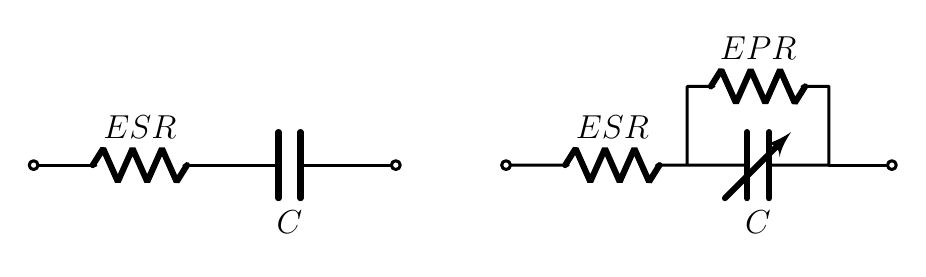
\begin{tikzpicture}
%Simple models of SCs
 %First Model (left)
	\coordinate (SC0) at (0,0) ;
	\draw (SC0) to [short,o-]++(0.4,0) to [R, l=$ESR$]++(1.9,0) to [C, l_=$C$]++(1.9,0) to [short,-o] ++(0.4,0);
%Second Model (right)
	\coordinate (SC1) at (6,0) ;
	\draw (SC1) to [short,o-]++(0.4,0) to [R, l=$ESR$]++(1.9,0) coordinate (E2)
	to [short] ++(0,1) to [R, l=$EPR$] ++(1.8,0) to [short] ++(0,-1) coordinate (C2) to [vC, invert,mirror, l=$C$](E2);% using "mirror" and "invert" one can change the direction of the arrow.
	\draw (C2) to [short, -o]++(0.8,0);
  \end{tikzpicture}
%
  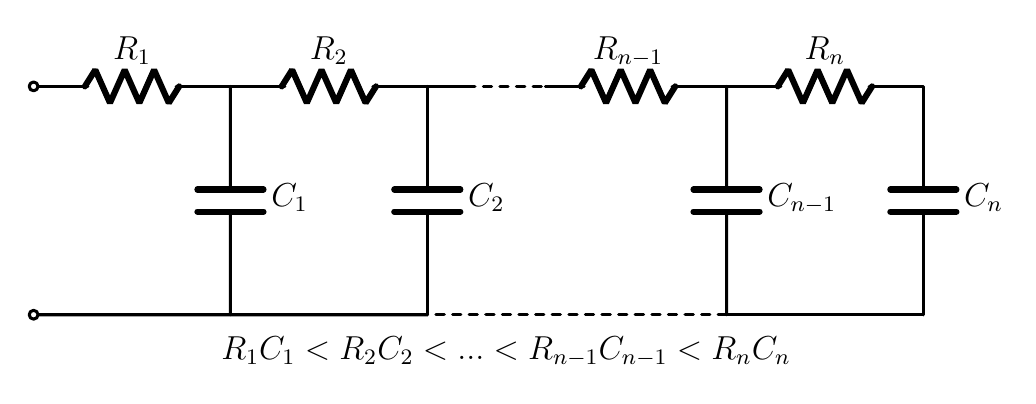
\begin{tikzpicture}
%Transmission line Model
	\newcommand\gap{0.2} %short gap between elements
	\newcommand\Rlength{2.1} %length of resistors
	\newcommand\Clength{2.9} %length of Capacitors
	\coordinate (SC0) at (0,0) ;
	\draw (SC0) to [short,o-]++(\gap,0) to [R, l=$R_{1}$]++(\Rlength,0) to [short]++(\gap,0) coordinate (C1T); %% C1T is the point from which capacitor1 will be
	\draw (C1T) to [short]++(\gap,0) to [R, l=$R_{2}$]++(\Rlength,0) to[short]++(\gap,0) coordinate (C2T); %% C2T is the point from which capacitor1 will be
	\draw (C2T) --++(0.5,0) coordinate (dashedT1); %% dashed line in the top part of the circuit
	\draw [dashed] (dashedT1) --++ (1,0) coordinate (dashedT2); %% where dashed finishes in the top
	\draw (dashedT2) to [R, l=$R_{n-1}$]++(\Rlength,0) to [short]++(\gap,0) coordinate (CN1T) to[short]++(\gap,0) to [R, l=$R_{n}$]++(\Rlength,0) to [short]++(\gap,0) to [C, l=$C_{n}$]++(0,-\Clength) coordinate (CnB); %% CnB is the bottom of Cn
	%CAPACITORS
	\draw (C1T) to [C, l=$C_{1}$]++(0,-\Clength) coordinate (C1B); %% C1B is the bottom of C1
	\draw (C2T) to [C, l=$C_{2}$]++(0,-\Clength) coordinate (C2B); %% C2B is the bottom of C2
	\draw (CN1T) to [C, l=$C_{n-1}$]++(0,-\Clength) coordinate (CN1B); %% CN1B is the bottom of CN1
	\draw (SC0) to [open,] ++(0,-\Clength) coordinate (SC0B) ; %% SC0B is the bottoom part of the input
	% Lines
	\draw (CnB) -- (CN1B);
	\draw [dashed] (CN1B) -- (C2B);
	\draw (C2B) -- (C1B) to [short,-o] (SC0B);
	%description
	\coordinate [label={[xshift=0, yshift=0] \large $R_{1}C_{1}<R_{2}C_{2} <...<R_{n-1}C_{n-1}<R_{n}C_{n}$ }] (des) at (6,-3.7) ;
  \end{tikzpicture}
%
  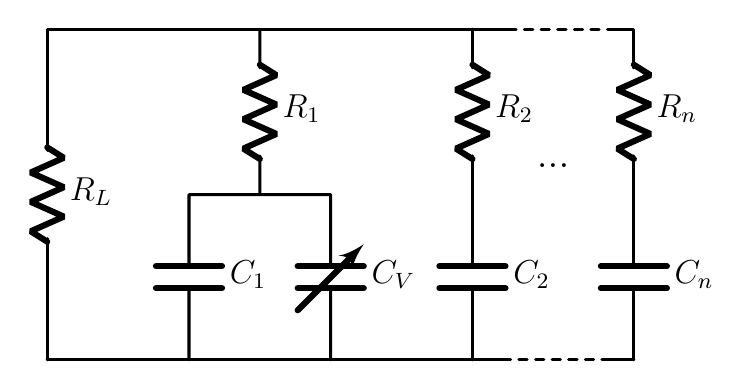
\begin{tikzpicture}
% Parallel model
	\newcommand\shortgap{0.9} %short gap between elements
	\newcommand\Rlength{2.1} %length of resistors
	\newcommand\Clength{2.9} %length of Capacitors
	\coordinate (SC0) at (0,0) ;
	\draw (SC0) to [R,l_=$R_{L}$] ++(0, 2*\Rlength) to [short] ++(3*\shortgap,0) coordinate (B2T); %% B2T is the top part of Branch 2
	\draw (B2T) to [R,l=$R_{1}$] ++(0, -\Rlength) coordinate (R1B) to [short] ++(-\shortgap,0) to [C, l=$C_{1}$] ++(0, -\Rlength) coordinate (C1B); %%R1B is bottom of the R1 and C1B is the top part of capacitor 1
	\draw (R1B) to [short]++(\shortgap,0) to [vC, invert, l=$C_{V}$] ++ (0,-\Rlength);
	\draw (B2T) to [short] ++(3*\shortgap,0) coordinate (B3T); %% B3T is the top part of Branch 3
	\draw (B3T)to [R,l=$R_{2}$]++ (0, -\Rlength) coordinate (mid1) to [C,l=$C_{2}$] ++ (0, -\Rlength) coordinate (B3B); %% B3B is the top part of Branch 3
	\draw (B3T) to [short] ++(0.5*\shortgap,0) coordinate (dashed1); %% dashed1 is the start of the dashed area
	\draw [dashed] (dashed1)--++(1.3,0) coordinate (dashed2); %% dashed 2 is the end of dashed area
	\draw (dashed2) to [short]++(0.3,0) to [R, l=$R_{n}$] ++(0, -\Rlength) coordinate (mid2) to [C, l=$C_{n}$]++(0,-\Rlength) coordinate (endd); %%endd is the end of the design
	\draw (endd) to [short]++(-0.3,0) coordinate (dashed2B);
	\draw [dashed] (dashed2B) -- ++(-1.3,0) coordinate (dashed1B);
	\draw (dashed1B) -- (SC0);
	\draw (mid1) to [open, l= \Large $...$] (mid2);
  \end{tikzpicture}
%
  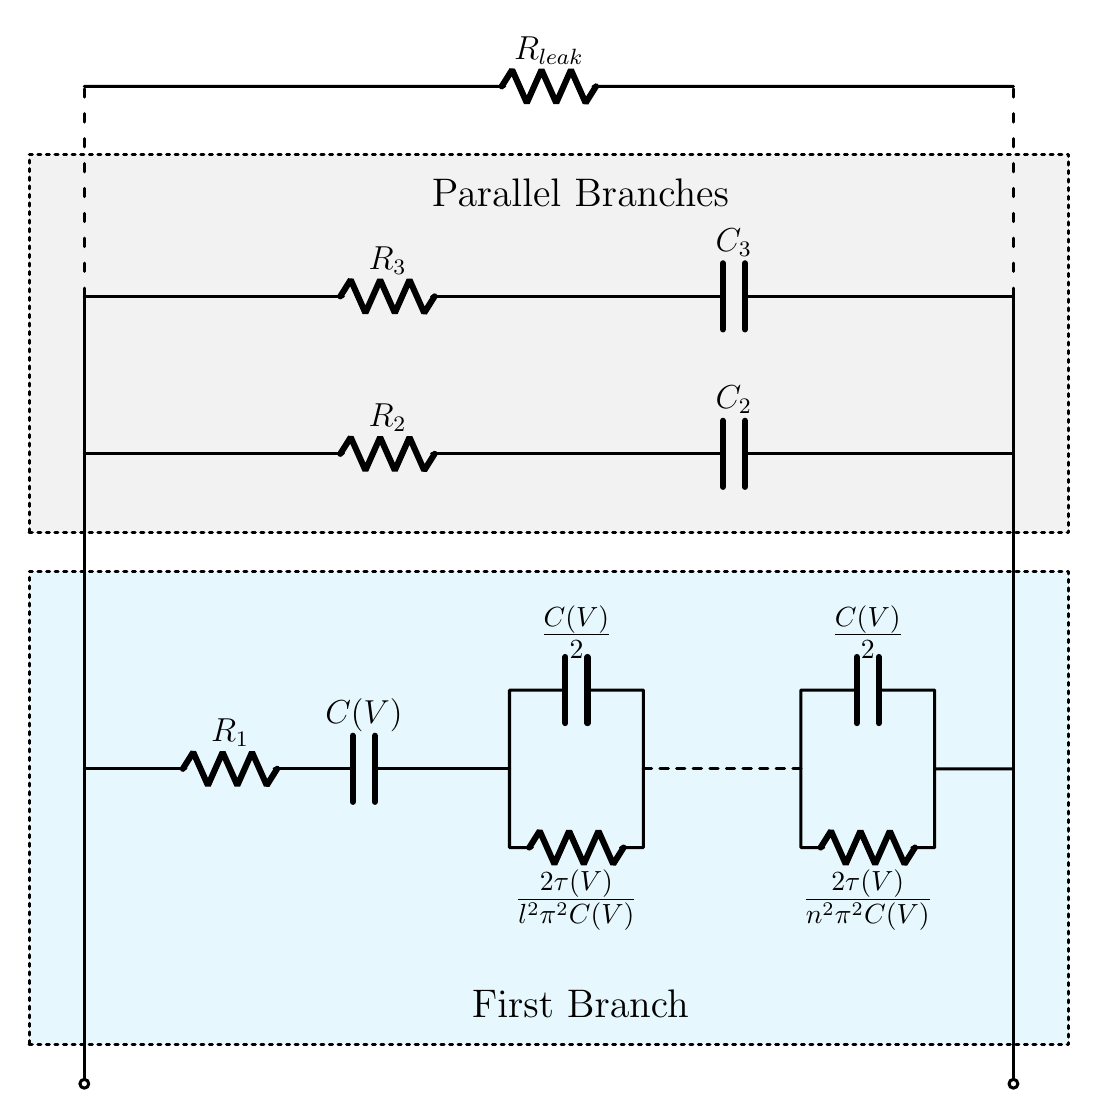
\begin{tikzpicture}
% Extended parallel model
	\newcommand\shgap{1} %short gap between elements
	\newcommand\Lgap{4} %large gap between elements
	\newcommand\Reslength{1.7} %length of resistors
	\newcommand\CapLength{1.7} %length of Capacitors
	\coordinate (SC0) at (0,0); %reference point 
	%Rectangle1
	\draw (SC0) ++ (-0.7,0.5) coordinate (RE1LB); %RE1LB= Rectangle 1 left bottom
	\draw (SC0) ++ (12.5, 0.5) coordinate (RE1RB); %RE1LB= Rectangle 1 Right bottom
	\draw (RE1LB) ++ (0,1.5* \Lgap) coordinate (RE1LT); %RE1LB= Rectangle 1 left top
	\draw (RE1RB) ++ (0, 1.5* \Lgap) coordinate (RE1RT); %RE1LB= Rectangle 1 Right top
	\draw [ dotted, fill=cyan!10] (RE1LB)-- (RE1RB)-- (RE1RT) --(RE1LT) -- cycle;
	% Rectangle2
	\draw (SC0) ++ (-0.7,7) coordinate (RE1LB); %RE1LB= Rectangle 1 left bottom
	\draw (SC0) ++ (12.5, 7) coordinate (RE1RB); %RE1LB= Rectangle 1 Right bottom
	\draw (RE1LB) ++ (0, 1.2* \Lgap) coordinate (RE1LT); %RE1LB= Rectangle 1 left top
	\draw (RE1RB) ++ (0, 1.2* \Lgap) coordinate (RE1RT); %RE1LB= Rectangle 1 Right top
	\draw [ dotted, fill=gray!10] (RE1LB)-- (RE1RB)-- (RE1RT) --(RE1LT) -- cycle;
	%First Branch
	\draw (SC0) --++(0,\Lgap) coordinate (B1L); %% B1L is the left side of the branch 1
	\draw (B1L) to [short]++(\shgap,0) to [R, l=$R_{1}$]++(\Reslength,0) to [C, l=$C(V)$] ++(\CapLength,0) to [short]++(\shgap,0) coordinate (P1L); % P1L is the left side of the first parallel branch.
	\draw (P1L) to [short] ++ (0,1) to [C, l= \Large $\frac{C(V)}{2}$] ++(\CapLength,0) to [short] ++ (0,-1) coordinate (P1R); %% P1R is the right side of the parallel branch
	\draw (P1L) to [short] ++ (0,-1) to [R, l_= \Large $\frac{2\tau (V)}{l^{2} \pi ^{2} C(V)}$] ++(\CapLength,0) to [short] ++ (0,1);
	\draw [dashed] (P1R) --++(2,0) coordinate (P2L); % P1L is the left side of the first parallel branch.
	\draw (P2L) to [short] ++ (0,1) to [C, l= \Large $\frac{C(V)}{2}$] ++(\CapLength,0) to [short] ++ (0,-1) coordinate (P2R); %P2R is the right side of the second parallel branch
	\draw (P2L) to [short] ++ (0,-1) to [R, l_= \Large $\frac{2\tau (V)}{n^{2} \pi ^{2} C(V)}$] ++(\CapLength,0) to [short] ++ (0,1) to [short]++(1,0) coordinate (B1R); % B1R is the right side of the branch
	\draw (B1R) -- ++(0,-\Lgap) coordinate (SC1);
	\draw (SC0) to [open, o-o] (SC1);
	% Second Branch
	\draw (B1L)--++(0,\Lgap) coordinate (B2L); % B2L is the left side of the second branch
	\draw (B1R)--++(0,\Lgap) coordinate (B2R); % B2R is the right side of the second branch
	\draw (B2L) to [short] ++(3*\shgap,0) to [R, l=$R_{2}$]++(\Reslength,0) to [C, l=$C_{2}$] (B2R);
	%Third Branch
	\draw (B2L)--++(0,\Lgap/2) coordinate (B3L); % B3L is the left side of the third branch
	\draw (B2R)--++(0,\Lgap/2) coordinate (B3R); % B3R is the right side of the third branch
	\draw (B3L) to [short] ++(3*\shgap,0) to [R, l=$R_{3}$]++(\Reslength,0) to [C, l=$C_{3}$] (B3R);
	%Fourth Branch
	\draw [loosely dashed] (B3L)--++(0,\Lgap/1.5) coordinate (B4L); % B4L is the left side of the fourth branch
	\draw [loosely dashed] (B3R)--++(0,\Lgap/1.5) coordinate (B4R); % B4R is the right side of the fourth branch
	\draw (B4L) to [R, l=$R_{leak}$] (B4R);
	%Descriptions
	\coordinate [ label={ \Large First Branch}] (DES1) at (6.3,0.7);
	\coordinate [ label={ \Large Parallel Branches }] (DES1) at (6.3,11);
  \end{tikzpicture}
\end{document}